%&pdflatex
\documentclass[
aps,%
12pt,%
final,%
notitlepage,%
oneside,%
onecolumn,%
nobibnotes,%
nofootinbib,%
superscriptaddress,%
noshowpacs,%
centertags]%
{revtex4}

\usepackage{wrapfig}

\usepackage[caption=false]{subfig}

\PassOptionsToPackage{monochrome}{xcolor}
\usepackage{tikz}
\usepackage{pgfplots}

\newcommand{\Kn}{\mathrm{Kn}}
\newcommand{\Ma}{\mathrm{M}}
\newcommand{\dd}{\:\mathrm{d}}
\newcommand{\pder}[2][]{\frac{\partial#1}{\partial#2}}
\newcommand{\pderder}[2][]{\frac{\partial^2 #1}{\partial #2^2}}
\newcommand{\Pder}[2][]{\partial#1/\partial#2}
\newcommand{\dzeta}{\boldsymbol{\dd\zeta}}
\newcommand{\bzeta}{\boldsymbol{\zeta}}
\newcommand{\Nu}{\mathcal{N}}
\newcommand{\OO}[1]{O\left(#1\right)}
\newcommand{\Set}[2]{\{\,{#1}:{#2}\,\}}

\begin{document}
\selectlanguage{russian}

\title{О медленных неизотермических течениях газа}
\author{\firstname{О.~А.}~\surname{Рогозин}}
\email{oleg.rogozin@phystech.edu}
\affiliation{Moсковский физико-технический институт}

\date{\today}

\begin{abstract}
    \begin{flushright}
    \vspace{1em}
    {\it Памяти Оскара Гаврииловича Фридлендера (1939--2015)}
    \vspace{1em}
    \end{flushright}
    Рассматриваются течения слаборазреженного газа
    под действием значительных температурных напряжений
    при условии, что число Рейнольдса порядка единицы.
    Предлагается оригинальный метод постановки граничных условий,
    позволяющий на основе уравнений гидродинамического типа
    получить приближённое решение для малых чисел Кнудсена,
    учитывающее температурный скачок возле границ обтекаемых тел.
    Метод апробирован на нескольких примерах.
    Результаты подкреплены прямым численным решением уравнения Больцмана
    на основе проекционного метода дискретных скоростей.
\end{abstract}

\keywords{
    уравнение Больцмана,
    температурные напряжения,
    неизотермические течения,
    асимптотический анализ,
    проекционный метод
}

\maketitle

%%%%%%%%%%%%%%%%%%%%%%%%%%%%%%%%%%%%%%%%%%%
\section{Введение}
%%%%%%%%%%%%%%%%%%%%%%%%%%%%%%%%%%%%%%%%%%%

С 1969 по 1974 год Оск\'{а}р Гавриилович Фридлендер (1939--2015)
совместно с Владленом Сергеевичем Галкиным (род.~1932)
под руководством Михаила Наумовича Когана (1925--2011)
развили теорию \emph{медленных неизотермических}
течений газа~\cite{Kogan1970, Kogan1971, Kogan1972, Friedlander1974, Kogan1976}.
Медленность течений следует понимать как малость числа Маха (\(\Ma\ll1\)),
а неизотермичность как присутствие в газе существенного градиента температур.
Основным импульсом упомянутых работ стала попытка учесть влияние температурных напряжений
на конвекцию газа через анализ барнеттовского приближения для слаборазреженного газа.
Несмотря на то что барнеттовские члены второго порядка малости по числу Кнудсена \(\Kn\),
при \(\Ma\sim\Kn\) они становятся сравнимыми с ньютоновскими вязкостными напряжениями.
Таким образом, уравнения Навье"--~Стокса оказываются некорректными для
описания медленных неизотермических течений.

В~\cite{Kogan1970} впервые была получена система уравнений гидродинамического типа,
адекватно описывающая медленные неизотермические течения слаборазреженного газа.
В литературе нет единого устоявшегося их названия,
поэтому автор предлагает ввести термин \emph{уравнения Когана"--~Галкина"--~Фридлендера}
или \emph{уравнения КГФ}.
Нелинейный характер температурных напряжений в полученных уравнениях приводит к
явлению конвекции газа под их действием~\cite{Kogan1971}.
Этот тип конвекции имеет место в отсутствие внешних сил и может возникать между равномерно нагретыми телами.
Нелинейные температурные напряжения при некоторых условиях влияют также на процессы теплопередачи~\cite{Friedlander1978}.
В результате многолетнего труда под руководством О.\,Г. Фридлендера теория медленных неизотермических течений
была подтверждена экспериментально~\cite{Friedlander1997, Friedlander2003}.
В это же время, благодаря развитию вычислительной техники, появилась возможность провести численные расчёты
некоторых прикладных задач с помощью уравнений КГФ, а также подтвердить асимптотику на основе модельного уравнения
Больцмана"--~Крука"--~Веландера (БКВ)~\cite{Alexandrov2002, Aoki2006, Alexandrov2008b, Alexandrov2011}
и прямого статистического моделирования (DSMC)~\cite{Alexandrov2008a, Aoki2007}.
Рассматривались также задачи с граничными условиями газ"--~жидкость,
учитывающие процессы испарения и конденсации~\cite{Aoki2007}.
Недавно теория была обобщена для смесей многоатомных газов~\cite{Galkin2015}.

В работах~\cite{Kogan1970,Kogan1971,Kogan1976} уравнения КГФ были получены наиболее простым способом,
на основе разложения Чепмена"--~Энскога, а необходимые транспортные коэффициенты были
вычислены в первом приближении с помощью полиномов Сонина~\cite{Chapman1960}.

Вывод уравнений КГФ различными способами:

Галкин В.С., Коган М.Н. К выводу уравнений медленных неизотермических течений газа. МЖГ. 1979, №6, 77-84.
Галкин В.С. Вывод уравнений медленных неизотермических течений смесей газов из уравнения Больцмана. Уч. зап. ЦАГИ. 1974, т.5б, №4, 40-47.

Строгий асимптотический анализ уравнения Больцмана для медленных неизотермических течений
на основе разложения Гильберта был впервые выполнен в~\cite{Sone1996},
а транспортные коэффициенты были пересчитаны прямыми численными методами с высокой точностью.
Несмотря на то что оба метода приводят к одинаковым системам уравнений ведущего порядка,
подход Гильберта позволяет изучить асимптотические свойства решения уравнений КГФ.
В частности, в~\cite{Sone1996} было показано, что в континуальном пределе (\(\Kn\to0\))
скоростное поле первого порядка конечным образом влияет на температурное распределение нулевого порядка.
Подобные \emph{призрак-эффекты} не проявляются в уравнениях Навье"--~Стокса с граничным условием без скольжения,
но впоследствии были обнаружены при асимптотическом анализе ряда других задач~\cite{Sone2007}.
Некоторые математические вопросы существования и гладкости решений уравнений КГФ обсуждаются,
например, в~\cite{Tan2016}.

В приведённых выше работах температурное поле нулевого порядка находилось из уравнений КГФ,
однако попытки получить приближение первого порядка малости от \(\Kn\) в литературе не встречаются.
Кроме того, в области малых \(\Kn\) нет достаточно точных решений уравнения Больцмана.
Распространённый метод DSMC, из-за присущих ему значительных флуктуаций, плохо пригоден
для медленных течений, особенно при малых \(\Kn\). В неизотермических течениях ситуация
ещё более усложняется, поскольку, в силу призрак-эффекта, ошибка \(\varepsilon\)
при вычислении поля скоростей приводит к ошибке порядка \(\varepsilon/\Kn\) при вычислении поля температур.

%%%%%%%%%%%%%%%%%%%%%%%%%%%%%%%%%%%%%%%%%%%
\section{Основные уравнения}
%%%%%%%%%%%%%%%%%%%%%%%%%%%%%%%%%%%%%%%%%%%

Прежде всего, перейдём к безразмерным переменным.
Пусть \(L\) "--- характерная длина в рассматриваемой задаче,
а \(T^{(0)}\) и \(p^{(0)}\) "--- характерные температура и давление газа.
Тогда макроскопические переменные принимают следующий вид:
температура \(TT^{(0)}\), давление \(pp^{(0)}\),
плотность \(\rho p^{(0)}/RT^{(0)}\), скорость \(v_i(2RT^{(0)})^{1/2}\).
Функция распределения молекулярных скоростей \(f(x_i,\zeta_i)(2p^{(0)})/(2RT^{(0)})^{5/2}\)
определяется в физическом пространстве \(x_iL\) и скоростном \(\zeta_i(2RT^{(0)})^{1/2}\).
Удельная газовая постоянная \(R = k_B/m\), где \(k_B\) "--- постоянная Больцмана,
\(m\) "--- молярная масса.
Число Кнудсена \(\Kn = \ell^{(0)}/L\) определяется через характерную длину свободного пробега
\begin{equation}\label{eq:ell}
    \ell^{(0)} = \frac{k_B T^{(0)}}{\sqrt2\pi d_m^2 p^{(0)}},
\end{equation}
где радиус действия межмолекулярного потенциала взаимодействия \(d_m\)
совпадает с диаметром молекул для модели твёрдых сфер.

Стационарное уравнение Больцмана в присутствии внешней силы \(F_i (2RT^{(0)})/L\) в безразмерных переменных имеет вид:
\begin{equation}\label{eq:Boltzmann}
    \zeta_i\pder[f]{x_i} + F_i\pder[f]{\zeta_i} = \frac1k J(f,f),
\end{equation}
где интеграл столкновений
\begin{equation}\label{eq:integral}
    J(f,g) = \frac12 \int(f'g'_*+g'f'_*-fg_*-gf_*)B\dd\Omega(\boldsymbol\alpha) \dzeta_*
\end{equation}
и \(k = \sqrt\pi\Kn/2\).
\(\Omega(\boldsymbol{\alpha})\) "--- телесный угол в направлении единичного вектора \(\boldsymbol\alpha\),
\(B\) "--- функционал межмолекулярного потенциала. Для модели твёрдых сфер,
\begin{equation}\label{eq:ci_kernel}
    B = \frac{|\alpha_i(\zeta_{i*}-\zeta_i)|}{4\sqrt{2\pi}}.
\end{equation}
Макроскопические переменные выражаются через моменты функции распределения:
\begin{equation}\label{eq:macro}
    \rho = \int f \dzeta, \quad
    v_i = \frac1{\rho} \int \zeta_i f \dzeta, \quad
    T = \frac{2}{3\rho}\int(\zeta_i-v_i)^2 f \dzeta, \quad
    p = \rho T.
\end{equation}

Граничные условия диффузного отражения задаются следующим образом:
\begin{equation}\label{eq:diffuse_bc}
    f\left(\zeta_i n_i > 0\right) =
        \frac{\sigma_B}{(\pi T_B)^{3/2}} \exp\left(-\frac{\zeta_i^2}{T_B}\right), \quad
    \sigma_B = -2\left(\frac{\pi}{T_B}\right)^{1/2} \int_{\zeta_i n_i < 0} \zeta_j n_j f\dzeta,
\end{equation}
где \(n_i\) "--- единичный вектор нормали к границе, направленный внутрь газа,
а \(T_B\) и \(v_{Bi}\) "--- граничные температура и скорость.
Для стационарных задач предполагается, что \(v_{Bi}n_i = 0\).

%%%%%%%%%%%%%%%%%%%%%%%%%%%%%%%%%%%%%%%%%%%
\section{Асимптотический анализ}
%%%%%%%%%%%%%%%%%%%%%%%%%%%%%%%%%%%%%%%%%%%

В этом разделе рассматривается асимптотическая теория,
подробное изложение которой можно найти
в~\cite{Sone1996, Sone2002, Sone2007}.
Для простоты рассматривается единственный потенциал межмолекулярного взаимодействия "---
модель твёрдых сфер.

\subsection{Система уравнений гидродинамического типа}

Функция распределения \(f(x_i,\zeta_i)\) и макроскопические переменные \(h = \rho, v_i, T, \dots\)
могут быть разложены в ряд по \(k\):
\begin{equation}\label{eq:expansion}
    f = f_0 + f_1k + f_2k^2 + \cdots, \quad h = h_0 + h_1k + h_2k^2 + \cdots.
\end{equation}
Если предположить, что \(\Pder[f]{x_i} = \OO{f}\) (разложение Гильберта),
\(v_{i0} = 0\) (медленные течения), \(F_{i0} = F_{i1} = 0\) (слабое поле внешних сил)
и подставить~\eqref{eq:expansion} в уравнение Больцмана~\eqref{eq:Boltzmann},
то для получаемых интегро-дифференциальных уравнений должны выполняться
условия разрешимости в нулевом порядке:
\begin{equation}
    \pder[p_0]{x_i} = 0, \label{eq:asymptotic0_p}
\end{equation}
в первом:
\begin{gather}
    \pder{x_i}\left(\frac{u_{i1}}{T_0}\right) = 0, \label{eq:asymptotic1_u} \\
    \pder[p_1]{x_i} = 0, \label{eq:asymptotic1_p} \\
    \frac{u_{i1}}{T_0}\pder[T_0]{x_i}
        = \frac{\gamma_2}2\pder{x_i}\left(\sqrt{T_0}\pder[T_0]{x_i}\right), \label{eq:asymptotic1_T} \\
\end{gather}
и во втором:
\begin{gather}
    \pder{x_i}\left(\frac{u_{i2}}{T_0}\right)
        + \pder{x_i}\left[\left(\frac{p_1}{p_0}-\frac{T_1}{T_0}\right)\frac{u_{i1}}{T_0}\right] = 0, \label{eq:asymptotic2_u} \\
    \begin{aligned}
    \pder{x_j}\left(\frac{u_{i1}u_{j1}}{T_0}\right)
        &-\frac{\gamma_1}2\pder{x_j}\left[\sqrt{T_0}\left(
            \pder[u_{i1}]{x_j} + \pder[u_{j1}]{x_i} - \frac23\pder[u_{k1}]{x_k}\delta_{ij}
        \right)\right] \\
        &- \frac{\gamma_7}{T_0}\pder[T_0]{x_i}\pder[T_0]{x_j}\left(\frac{u_{j1}}{\gamma_2\sqrt{T_0}} - \frac{1}4\pder[T_0]{x_j}\right)
        = -\frac12\pder[p_2^\dag]{x_i} + \frac{p_0^2 F_{i2}}{T_0},
    \end{aligned} \label{eq:asymptotic2_p} \\
    \frac{u_{i1}}{T_0}\pder[T_1]{x_i}
        + \left[\frac{u_{i2}}{T_0} + \left(\frac{p_1}{p_0}-\frac{T_1}{T_0}\right)\frac{u_{i1}}{T_0}\right]\pder[T_0]{x_i}
        = \frac{\gamma_2}2\pder{x_i}\left(\sqrt{T_0}\pder[T_1]{x_i} + \frac{T_1}{2\sqrt{T_0}}\pder[T_0]{x_i}\right). \label{eq:asymptotic2_T}
\end{gather}
Здесь обозначены \(u_{i1} = p_0v_{i1}\), \(u_{i2} = p_0v_{i2}\) и
\begin{equation}\label{eq:dag_pressure}
    p_2^\dag = p_0 p_2
        + \frac{2\gamma_3}{3}\pder{x_k}\left(T_0\pder[T_0]{x_k}\right)
        - \frac{\gamma_7}{6}\left(\pder[T_0]{x_k}\right)^2.
\end{equation}
Уравнения~\eqref{eq:asymptotic1_u},~\eqref{eq:asymptotic1_T},~\eqref{eq:asymptotic2_p}
для \(T_0\), \(u_{i1}\) и \(p_2^\dag\) будем называть уравнениями КГФ
в соответствии с пионерскими работами~\cite{Kogan1992, Bobylev1995}.
Они содержат член температурных напряжений, отсутствующий в уравнениях Навье"--~Стокса.
Сравнивая его с \(p_0^2F_{i2}/T_0\), можно увидеть, что на единицу массы действует сила
\begin{equation}\label{eq:gamma7_force}
    k^2\frac{\gamma_7}{p_0^2}\pder[T_0]{x_i}\pder[T_0]{x_j}\left(\frac{u_{j1}}{\gamma_2\sqrt{T_0}} - \frac{1}4\pder[T_0]{x_j}\right).
\end{equation}
Для модели твёрдых сфер, эта сила противоположна градиенту температур.
Важно отметить, что \(p_2^\dag\) не входит в уравнение состояния,
поэтому определяется с точностью до константы.
Поскольку член \(\partial{p_2^\dag}/\partial{x_i}\) включён в систему,
как давление в уравнениях Навье"--~Стокса для несжимаемого газа,
то для решения уравнений КГФ применяются соответствующие численные методы.

Безразмерные транспортные коэффициенты для модели твёрдых сфер равны
\begin{alignat*}{2}\label{eq:gamma_coeffs}
    \gamma_1 &= 1.270042427, &\quad \gamma_2 &= 1.922284066, \\
    \gamma_3 &= 1.947906335, &\quad \gamma_7 &= 1.758705.
\end{alignat*}
Первые два коэффициента соответствуют вязкости \(\mu\) и теплопроводности \(\lambda\) газа, т.е.
\begin{equation}\label{eq:mu_lambda}
    \mu = \gamma_1\sqrt{T_0} \frac{p^{(0)}L}{\sqrt{2RT^{(0)}}} k, \quad
    \lambda = \frac{5\gamma_2}{2}\sqrt{T_0} \frac{p^{(0)}RL}{\sqrt{2RT^{(0)}}} k.
\end{equation}
Коэффициент \(\gamma_3\) входит в значения температурных напряжений,
которые создают неоднородное распределение давления в газе,
но не движущую силу. Коэффициент \(\gamma_7\) соответствует
температурной конвекции газа.

\subsection{Граничные условия}

Граничные условия диффузного отражения имеют вид:
\begin{gather}
    T_0 = T_{B0}, \label{eq:bc_T0} \\
    T_1 = T_{B1} + d_1\frac{T_{B0}}{p_0}\pder[T_0]{x_j} n_j, \label{eq:bc_T1} \\
    \left\{
    \begin{aligned}
        & u_{j1} (\delta_{ij}-n_in_j) =
            \left(u_{Bj1} - K_1 \sqrt{T_{B0}} \pder[T_0]{x_j}\right) (\delta_{ij}-n_in_j), \\
        & u_{j1} n_j = 0.
    \end{aligned}
    \right. \label{eq:bc_u1}
\end{gather}
Здесь \(d_1\) "--- коэффициент температурного скачка, а \(K_1\) "--- коэффициент теплового скольжения.
Для модели твёрдых сфер,
\begin{equation}\label{eq:slip_coefficients}
    d_1 = 2.4001, \quad K_1 = -0.6463.
\end{equation}

Решение уравнений КГФ не удовлетворяет в общем случае кинетическому граничному условию~\eqref{eq:diffuse_bc}
поскольку функция распределения изменяется значительно вблизи границы вдоль нормали к ней.
Коррекция макроскопических переменных \(h = h_0 + (h_1 + h_{K1})k + \cdots\) в кнудсеновском слое
принимает следующий вид:
\begin{gather}
    T_{K1} = \frac{T_{B0}}{p_0}\left.\pder[T_0]{x_j}\right|_0 n_j
        \Theta_1\left(\frac{p_0}{T_{B0}}\eta\right), \label{eq:correction_T} \\
    \rho_{K1} = \frac1{T_{B0}}\left.\pder[T_0]{x_j}\right|_0 n_j
        \Omega_1\left(\frac{p_0}{T_{B0}}\eta\right), \label{eq:correction_rho} \\
    \left\{
    \begin{aligned}
        & u_{jK1} (\delta_{ij}-n_in_j) =
            -\frac{\sqrt{T_{B0}}}2 \left.\pder[T_{B0}]{x_j}\right|_0
            Y_1\left(\frac{p_0}{T_{B0}}\eta\right) (\delta_{ij}-n_in_j), \\
        & u_{jK1} n_j = 0,
    \end{aligned}
    \right. \label{eq:correction_u}
\end{gather}
где \(\eta = (x_i-x_{Bi})n_i/k\), \(x_{Bi}\) "--- ближайшая к \(x_i\) точка на границе,
а \(|_0\) означает значение на границе (\(\eta=0\)).
Функции \(\Theta_1(\eta)\), \(\Omega_1(\eta)\), \(Y_1(\eta)\) убывают экспоненциально от \(\eta\)
и табулированы для модели твёрдых сфер в~\cite{Sone2002, Sone2007}.

Разложение в ряд граничной температуры \(T_B = T_{B0} + T_{B1}k + \cdots\) может быть выполнено
произвольным образом. Обычно полагают, что \(T_{B1}=0\)~\cite{Kogan1976, Sone1996},
что позволяет получить температурное поле с точностью \(\OO{k}\).
Если же положить, что \(T_1=0\) на границе,
тогда из~\eqref{eq:bc_T0} и~\eqref{eq:bc_T1} следует,
что \(T_0\) вычисляется из уравнения
\begin{equation}\label{eq:boundary_temp}
    T_B = T_0 \left( 1 - \frac{d_1}{p_0}\pder[T_0]{x_j}n_j k \right).
\end{equation}
При таком граничном условии получается приближённое решение,
для которого температура газа на границе вычисляется с точностью \(\OO{k^2}\).
Однако из уравнения~\eqref{eq:asymptotic2_T} видно, что в общем случае во всей области
решение обладает точностью \(\OO{k}\).

\subsection{Континуальный предел}

Рассмотрим поведение системы уравнений КГФ~\eqref{eq:asymptotic1_u},~\eqref{eq:asymptotic1_T},~\eqref{eq:asymptotic2_p}
в континуальном пределе (\(k\to0\)).
Поле скоростей \(v_i\) стремится к нулю, поскольку \(v_{i0}=0\),
однако скорость \(v_{i1}\), которая вносит инфинитезимальный вклад в \(v_i\),
конечным образом влияет на \(T_0\).
Такое асимптотическое поведение получило название \emph{призрак-эффекта} (ghost effect)~\cite{Sone2002, Sone2007}.

Можно выделить три причины возникновения конечного поля \(v_{i1}\).
Во-первых, если граница движется со скоростью \(v_{B1}\ne0\).
Во-вторых, если на границе присутствует градиент температуры \(\Pder[T_0]{x_i}\ne0\) (эффект \emph{теплового скольжения}).
В-третьих, когда изотермические поверхности не параллельны
\begin{equation}\label{eq:nonparallel}
    e_{ijk}\pder[T_0]{x_j}\pder{x_k}\left(\pder[T_0]{x_l}\right)^2 \ne 0,
\end{equation}
возникает конвекция газа под действием температурных напряжений (\emph{термострессовая конвекция}).

В классической гидродинамике, уравнения Навье"--~Стокса (\(\gamma_7=0\))
с неподвижными (\(v_B=0\)) граничными условиями без скольжения (\(K_1=0\), \(d_1=0\))
приводят к нулевому полю \(v_{i1} = 0\) и к уравнению теплопроводности
\begin{equation}\label{eq:heat_equation}
    \pder{x_i}\left(\sqrt{T_0}\pder[T_0]{x_i}\right) = 0.
\end{equation}
Тем не менее, для корректного описания в континуальном пределе температурного поля \(T\equiv T_0\)
необходимо решать уравнения КГФ~\eqref{eq:asymptotic1_u},~\eqref{eq:asymptotic1_T},~\eqref{eq:asymptotic2_p}
с соответствующими граничными условиями~\eqref{eq:bc_T0},~\eqref{eq:bc_u1}.

%%%%%%%%%%%%%%%%%%%%%%%%%%%%%%%%%%%%%%%%%%%
\section{Метод решения уравнения Больцмана}
%%%%%%%%%%%%%%%%%%%%%%%%%%%%%%%%%%%%%%%%%%%

В настоящей работе уравнение Больцмана решается численно с помощью
симметричного расщепления на уравнение переноса
\begin{equation}\label{eq:split_advection}
    \pder[f]{t} + \zeta_i\pder[f]{x_i} = 0,
\end{equation}
для которого используется метод конечных объёмов с явной TVD-схемой второго порядка,
и однородное уравнение Больцмана
\begin{equation}\label{eq:split_integral}
    \pder[f]{t} = \frac1k J(f,f),
\end{equation}
для которого используется проекционно-интерполяционный метод дискретных скоростей~\cite{Tcheremissine1997, Tcheremissine2006}.
Несмотря на то что проекционный метод обладает вторым порядком аппроксимации в пространстве скоростей~\cite{Anikin2012},
в граничных задачах медленных течений возникают разрывы функции распределения скоростей.
Таким образом, для получения адекватной аппроксимации в слое Кнудсена необходимо прибегать
к измельчению сетки вблизи линии разрыва.
Далее коротко описывается методика консервативного вычисления интеграла столкновений Больцмана
для произвольной прямоугольной сетки в пространстве скоростей.

%%% Numerical approximation
Пусть регулярная скоростная сетка построена таким образом,
что кубатура в пространстве \(\bzeta\) выражается в виде взвешенной суммы
\begin{equation}\label{eq:zeta_cubature}
    \int F(\bzeta) \dzeta \approx \sum_{\gamma\in\Gamma} F_\gamma w_\gamma,
        \quad \sum_{\gamma\in\Gamma} w_\gamma = V_\Gamma,
        \quad F_\gamma = F(\bzeta_\gamma),
\end{equation}
где \(\mathcal{V} = \Set{\zeta_\gamma}{\gamma\in\Gamma}\) "--- множество дискретных скоростей,
\(F\) "--- произвольная функция от \(\bzeta\),
а \(V_\Gamma\) "--- общий объём скоростной сетки.
Тогда интеграл столкновений, записанный в симметризованной форме
\begin{equation}\label{eq:symm_ci}
    \begin{aligned}
    J(f_\gamma, f_\gamma) = \frac14\int &\left[
        \delta(\bzeta-\bzeta_\gamma) + \delta(\bzeta_*-\bzeta_\gamma)
        - \delta(\bzeta'-\bzeta_\gamma) - \delta(\bzeta'_*-\bzeta_\gamma)\right] \\
        &\times(f'f'_* - ff_*)B \dd\Omega(\boldsymbol{\alpha}) \dzeta\dzeta_*,
    \end{aligned}
\end{equation}
где \(\delta(\bzeta)\) "--- дельта-функция Дирака в \(\mathbb{R}^3\),
имеет следующий дискретный аналог:
\begin{equation}\label{eq:discrete_symm_ci}
    \hat{J}_\gamma = \frac{\pi V_\Gamma^2}{\sum_{\nu\in\Nu} w_{\alpha_\nu}w_{\beta_\nu}}
        \sum_{\nu\in\Nu} \left(
            \delta_{\alpha_\nu\gamma} + \delta_{\beta_\nu\gamma}
            - \delta_{\alpha'_\nu\gamma} - \delta_{\beta'_\nu\gamma}
        \right)\left(
            \frac{w_{\alpha_\nu}w_{\beta_\nu}}{w_{\alpha'_\nu}w_{\beta'_\nu}}
            \hat{f}_{\alpha'_\nu}\hat{f}_{\beta'_\nu} - \hat{f}_{\alpha_\nu}\hat{f}_{\beta_\nu}
        \right)B_\nu.
\end{equation}
Здесь \(\alpha_\nu\in\Gamma\) и \(\beta_\nu\in\Gamma\), наряду с \(\boldsymbol{\alpha}_\nu\),
берутся по правилу Коробова~\cite{Korobov1959, Sloan1994} для восьмимерной кубатуры.
Кроме того, кубатурная решетка случайным образом сдвигается на каждом шаге по времени.
Модифицированная функция распределения \(\hat{f}_\gamma = f_\gamma w_\gamma\) используется для удобства.
Дискретный аналог распределения Максвелла может быть записан в следующем виде:
\begin{equation}\label{eq:discrete_Maxwell}
    \hat{f}_{M\gamma} = \rho\left[\sum_{\alpha\in\Gamma}w_\alpha\exp
            \left(-\frac{(\bzeta_\alpha - \boldsymbol{v})^2}{T}\right)
        \right]^{-1}
        w_\gamma\exp\left(-\frac{(\bzeta_\gamma - \boldsymbol{v})^2}{T}\right).
\end{equation}

%%% Projection and interpolation
В общем случае, скорости после столкновения,
\(\bzeta_{\alpha'_\nu}\) и \(\bzeta_{\beta'_\nu}\), не попадают в \(\mathcal{V}\).
Если они просто заменяются ближайшими сеточными скоростями,
\(\bzeta_{\lambda_\nu}\in\mathcal{V}\) и \(\bzeta_{\mu_\nu}\in\mathcal{V}\),
дискретный интеграл столкновений~\eqref{eq:discrete_symm_ci} теряет свойство консервативности.
Более того, дискретное распределение Максвелла~\eqref{eq:discrete_Maxwell} перестаёт быть равновесным состоянием.
Для решения этих проблем в проекционно-интерполяционном методе применяются следующие две процедуры.
Во-первых, \(\bzeta_{\alpha'_\nu}\) проецируется на \(\bzeta_{\lambda_\nu}\) и
на некоторое множество соседних узлов, \(\Set{\bzeta_{\lambda_\nu+s_a}}{a\in\Lambda}\subset\mathcal{V}\),
степенным образом:
\begin{equation}\label{eq:ci_projection}
    \delta_{\alpha'_\nu\gamma} = \sum_{a\in\Lambda} r_{\lambda,a}\delta_{\lambda_\nu+s_a,\gamma}.
\end{equation}
Веса \(r_{\lambda,a}\) выбираются так, чтобы обеспечить сохранение массы, импульса и энергии, т.е.
\begin{equation}\label{eq:impact_conservation}
    \sum_{a\in\Lambda} r_{\lambda,a} = 1, \quad
    \sum_{a\in\Lambda} r_{\lambda,a} \bzeta_{\lambda_\nu+s_a} = \bzeta_{\alpha'_\nu}, \quad
    \sum_{a\in\Lambda} r_{\lambda,a} \bzeta_{\lambda_\nu+s_a}^2 = \bzeta_{\alpha'_\nu}^2.
\end{equation}
Множество проекционных точек \(\mathcal{S}_{\alpha'_\nu} = \Set{\bzeta_{\lambda_\nu+s_a}}{a\in\Lambda, r_{\lambda,a}\neq0}\)
называется проекционным шаблоном.
Для равномерной сетки, достаточно двух проекционных точек для достижения консервативности,
в то время как для неравномерной сетки минимальный шаблон состоит из пяти точек, \(|\mathcal{S}_{\alpha'_\nu}|=5\).
Во-вторых, чтобы удовлетворить условию \(J_\gamma(\hat{f}_{M\gamma}, \hat{f}_{M\gamma}) = 0\),
\(\hat{f}_{\alpha'_\nu}\) интерполируется следующим образом:
\begin{equation}\label{eq:ci_interpolation}
    \frac{\hat{f}_{\alpha'_\nu}}{w_{\alpha'_\nu}} = \prod_{a\in\Lambda}
        \left(\frac{\hat{f}_{\lambda_\nu+s_a}}{w_{\lambda_\nu+s_a}} \right)^{r_{\lambda,a}}.
\end{equation}
Этот тип интерполяции требует высоких затрат с вычислительной точки зрения,
но для медленных течений, когда функция распределения близка к максвелловской,
позволяет добиться высокой точности и низкого уровня флуктуаций.
Для \(\bzeta_{\beta'_\nu}\) и \(\hat{f}_{\beta'_\nu}\) все формулы аналогичны.

%%% About excluding points
Существует ещё одно важное и необходимое свойство численного алгоритма:
функция распределения должна всегда оставаться положительной.
Если в сумме~\eqref{eq:discrete_symm_ci} присутствует член, нарушающий это свойство,
то его необходимо исключить из \(\mathcal{N}\).
С другой стороны, большое количество таких исключенных столкновений
нарушает кубатурную решетку, следовательно, существенно увеличивается ошибка аппроксимации.
Чтобы предотвратить такую ситуацию, необходимо либо уменьшить временной шаг, либо увеличить \(\mathcal{N}\).
Если мы предположим, что кубатурная решетка создаёт ошибку аппроксимации \(\OO{|\mathcal{N}|^{-1}}\),
то исключение \(M\) случайно распределённых узлов приводит к ошибке \(\OO{\sqrt{M}/|\mathcal{N}|}\).

%%%%%%%%%%%%%%%%%%%%%%%%%%%%%%%%%%%%%%%%%%%
\section{Численные примеры}
%%%%%%%%%%%%%%%%%%%%%%%%%%%%%%%%%%%%%%%%%%%

%%% SNIT solver
В настоящей работе уравнения КГФ~\eqref{eq:asymptotic1_u},~\eqref{eq:asymptotic1_T},~\eqref{eq:asymptotic2_p}
решаются с помощью солвера \verb+snitSimpleFoam+~\cite{Rogozin2014},
использующего метод конечных объёмов на основе вычислительной платформы OpenFOAM\textregistered{}.
В частности, реализован численный алгоритм, подобный распространёному методу SIMPLE~\cite{Aoki2007}.
%%% Boltzmann solver
Программная реализация описанного алгоритма численного решения уравнения Больцмана
осуществлена в рамках проблемно-моделирующей среды
для анализа газокинетических процессов~\cite{Kloss2011, Kloss2012}.

\subsection{Задача Соне"--~Бобылева}

\begin{wrapfigure}{r}{7.4cm}
    \vspace{-10pt}
    \centering
    \includegraphics{Fig01}
    \vspace{-20pt}
    \caption{Геометрия задачи}\label{fig:sone_bobylev}
    \vspace{20pt}
\end{wrapfigure}

Рассмотрим плоскую периодическую геометрию, как на рис.~\ref{fig:sone_bobylev}.
Газ расположен между двумя покоящимися (\(v_{Bi} = 0\)) бесконечными параллельными пластинами,
разделёнными на единичное расстояние. Их температура распределена на них по синусоидальному закону:
\begin{equation}
    T_B = 1 - \frac{\cos(2\pi x)}{2}.
\end{equation}
В качестве граничного условия на пластинах используется полное диффузное отражение.
Плотность газа нормирована на единицу, т.е.
\begin{equation}\label{eq:total_mass}
    \int_0^1\int_0^1\rho\dd{x}\dd{y} = 1.
\end{equation}

В силу симметрии задачи, расчётная область представляет собой квадрат со стороной \(1/2\).
На рис.~\ref{fig:sone_bobylev} выделена серым цветом.
Подобная задача изучалась в~\cite{Sone1996} как с помощью уравнений КГФ, так и на основе кинетического подхода,
однако из-за высокой сложности численного решения уравнения Больцмана, использовалось модельное уравнение БКВ.
В настоящей работе получено прямое решение уравнения Больцмана для модели твёрдых сфер.
Кроме того, в рамках задачи рассмотрим приближённое решение гидродинамического типа для малых \(\Kn\),
основанное на граничном условии~\eqref{eq:boundary_temp}.

\subsubsection{Решение задачи в континуальном пределе}

\begin{figure}
    %\centering
    \subfloat[уравнение теплопроводности~\eqref{eq:heat_equation}]{
        \includegraphics[width=0.5\textwidth]{Fig02}
        \label{fig:continuum:temp-heat}
    }
    \subfloat[уравнения КГФ]{
        \includegraphics[width=0.5\textwidth]{Fig03}
        \label{fig:continuum:temp-snit}
    }
    \caption{Изотермические линии в континуальном пределе}
    \label{fig:continuum:temp}
\end{figure}

\begin{figure}
    \centering
    \subfloat[уравнения КГФ без скольжения (\(K_1=0\))]{
        \includegraphics[width=0.5\textwidth]{Fig04}
        \label{fig:continuum:flow-nonslip}
    }
    \subfloat[уравнения КГФ]{
        \includegraphics[width=0.5\textwidth]{Fig05}
        \label{fig:continuum:flow-snit}
    }
    \caption{Стационарное поле \(v_{i1}\) в континуальном пределе:
        изолинии соответствуют модулю, кривые со стрелками изображают направление}
    \label{fig:continuum:flow}
\end{figure}

%%% Space discretization
Для численного решения поставленной задачи в физическом пространстве
используется следующая прямоугольная сетка:
область \(0<x<1/2\) разбивается на 30 интервалов одинаковой длины,
а область \(0<y<1/2\) на 40 интервалов, сгущающихся к \(y=0\).

%%% Results and discussions
На рис.~\ref{fig:continuum:temp} показано стационарное температурное поле,
получаемое как при решении уравнения теплопроводности, так и уравнений КГФ.
В континуальном пределе уравнение теплопроводности получается из уравнений КГФ,
если положить \(\gamma_7=0\) и \(K_1=0\).
Эффект теплового скольжения газа значительно превышает конвекцию под действием температурных напряжений,
что продемонстрированно на рис.~\ref{fig:continuum:flow}, где уравнения КГФ решены
для граничных условий со скольжением и без.
Отметим также, что направления течения газа противоположны на рис.~\ref{fig:continuum:flow-nonslip}
и~\ref{fig:continuum:flow-snit}.
Представленные в этой подсекции результаты полностью совпадают с представленными в~\cite{Sone1996}.
Этот факт может служить верификацией используемого солвера \verb+snitSimpleFoam+.

\subsubsection{Решение для произвольных чисел Кнудсена}

\begin{figure}
    \centering
    \subfloat[уравнения КГФ с граничным условием~\eqref{eq:boundary_temp}]{
        \includegraphics[width=0.5\textwidth]{Fig06}
        \label{fig:kn0.01:temp-snit}
    }
    \subfloat[уравнение Больцмана]{
        \includegraphics[width=0.5\textwidth]{Fig07}
        \label{fig:kn0.01:temp-exact}
    }
    \caption{Изотермические линии для \(\Kn=0.01\)}
    \label{fig:kn0.01:temp}
\end{figure}

\begin{figure}
    \centering
    \subfloat[уравнения КГФ с граничным условием~\eqref{eq:boundary_temp}]{
        \includegraphics[width=0.5\textwidth]{Fig08}
        \label{fig:kn0.01:flow-snit}
    }
    \subfloat[уравнение Больцмана]{
        \includegraphics[width=0.5\textwidth]{Fig09}
        \label{fig:kn0.01:flow-exact}
    }
    \caption{Стационарное поле скоростей для \(\Kn=0.01\):
        изолинии соответствуют модулю, кривые со стрелками изображают направление}
    \label{fig:kn0.01:flow}
\end{figure}

\begin{figure}
    \centering
    \subfloat[изотермические линии]{
        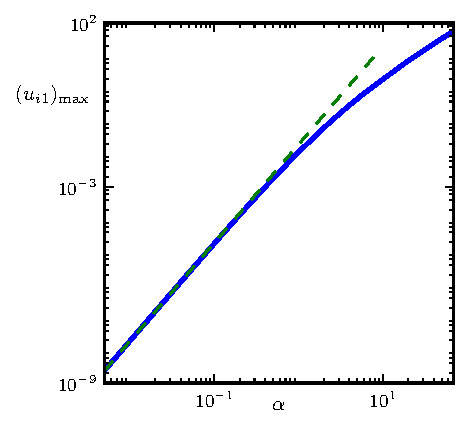
\includegraphics[width=0.5\textwidth]{Fig10}
        \label{fig:kn0.1:temp}
    }
    \subfloat[поле скоростей]{
        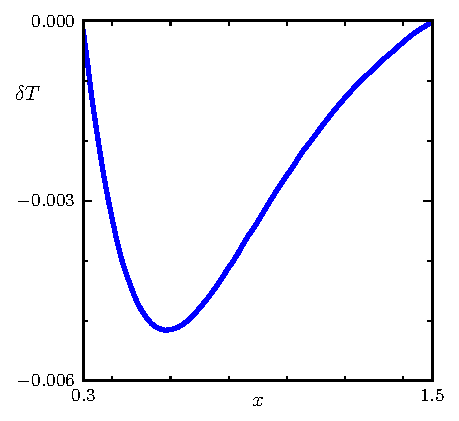
\includegraphics[width=0.5\textwidth]{Fig11}
        \label{fig:kn0.1:flow}
    }
    \caption{Решение уравнения Больцмана для \(\Kn=0.1\)}
    \label{fig:kn0.1}
\end{figure}

%%% Space discretization
Для рассмотрения задачи в произвольном диапазоне чисел Кнудсена необходимо
обратиться к численному решению уравнения Больцмана.
В физическом пространстве использовалась такая же разностная сетка,
как и при решении уравнений гидродинамического типа,
однако в слое Кнудсена (вблизи \(y=0\)) она дополнительно сгущалась так,
что ширина приграничной ячейки равнялась \(0.02\) от длины свободного пробега.
Для контроля точности использовались две различные сетки в скоростном пространстве.
Сначала задача решалась на равномерной прямоугольной сетке, ограниченной сферой радиусом \(4.24\),
так что на радиусе помещалось 8 ячеек.
Далее результат уточнялся на неравномерной сетке, ограниченной сферой радиусом \(5.3\),
причём вдоль осей \(x\) и \(z\) границы ячеек располагались как корни полинома Эрмита,
а вдоль оси \(y\) сгущались в геометрической прогрессии так,
что ширина ячеек возле \(y=0\) равнялась \(0.0067\).
Таким образом, на радиусе помещалось 9, 26, 9 ячеек соответственно.
Кубатурные сетки также имели разную мощность: около 5000 для равномерной сетки
и около 200000 для неравномерной.
Кроме того, для очень малых \(\Kn\) применялась временн\'{а}я экстраполяция распределения температуры
и поля скоростей, поскольку достижение стационарного состояния вблизи \(y=1/2\)
требует слишком большого числа итераций.

%%% Results and discussions
На рис.~\ref{fig:kn0.01:temp} и~\ref{fig:kn0.01:flow} изображено поле температуры и скорости
для \(\Kn=0.01\) и проводится сравнение между численным решением уравнения Больцмана
и приближённым решением для малых \(\Kn\).
На рис.~\ref{fig:kn0.1} показаны соответствующие распределения для \(\Kn=0.1\).
С увеличением \(\Kn\) возрастает поток теплового скольжения и температурный скачок возле границы \(y=0\).
При этом область максимальной скорости газа отодвигается от пластины.

\newcommand*{\graphlinewidth}{1}
\pgfplotscreateplotcyclelist{legend}{
    {cyan,  dashdotted, line width=\graphlinewidth},
    {blue,  solid,      line width=\graphlinewidth},
    {green, dashed,     line width=\graphlinewidth},
    {red,   dashed,     line width=\graphlinewidth, mark=o, mark options={solid}},
    {magenta, dotted,     line width=\graphlinewidth, mark=square, mark options={solid}},
}
\newcommand{\pgfplotsReferenceGenerator}[3]{
    \scalebox{0}{
        \begin{tikzpicture}
            \begin{axis}[hide axis, cycle list name = #1]
                \foreach \i   [evaluate=\i] in {1,...,#2}{
                    \addplot (0,0); \label{#3\i}
                }
            \end{axis}
        \end{tikzpicture}
    }
}

\pgfplotsReferenceGenerator{legend}{5}{line}

\begin{figure}
    \centering
    \subfloat[]{
        \includegraphics[width=0.5\textwidth]{Fig12}
        \label{fig:comparison:bottomT}
    }
    \subfloat[]{
        \includegraphics[width=0.5\textwidth]{Fig13}
        \label{fig:comparison:bottomU}
    }\\
    \subfloat[]{
        \includegraphics[width=0.5\textwidth]{Fig14}
        \label{fig:comparison:topT}
    }
    \subfloat[]{
        \includegraphics[width=0.5\textwidth]{Fig15}
        \label{fig:comparison:topU}
    }
    \caption{
        Некоторые пограничные интегралы в зависимости от \(\Kn\), полученные разными методами:
        уравнение теплопроводности~\ref{line1},
        уравнения КГФ с условием~\eqref{eq:boundary_temp}~\ref{line2} и без~\ref{line3},
        уравнение Больцмана на равномерной~\ref{line4} и неравномерной~\ref{line5} сетках
    }
    \label{fig:comparison}
\end{figure}

%%% Comparison between solutions
Чтобы наглядно продемонстрировать сходимость численного решения уравнения Больцмана к
решению уравнений КГФ в континуальном пределе, рассмотрим рис.~\ref{fig:comparison}.
На рис.~\ref{fig:comparison:topT} отчётливо видно, что решение уравнения Больцмана сходится
именно к решению уравнений КГФ, а не уравнения теплопроводности.
Для самых малых \(\Kn\) погрешность решения уравнения Больцмана возрастает
ввиду получения стационарного значения посредством экстраполяции.
На рис.~\ref{fig:comparison:bottomT} приближённое решение гидродинамического типа
на основе граничного условия~\eqref{eq:boundary_temp} аппроксимирует
точное решение со вторым порядком точности,
в то время как другие решения дают только первый порядок.
Приближённое решение отличается от точного менее чем на 10\% в области \(\Kn<0.05\),
однако стоит учитывать, что в рассматриваемой задаче тепловое скольжение значительно превалирует
над термострессовой конвекцией. Для противоположного случая приближённое решение может давать
б\'{о}льшую погрешность.

%%%%%%%%%%%%%%%%%%%%%%%%%%%%%%%%%%%%%%%%%%%
\subsection{Задача Фридлендера}
%%%%%%%%%%%%%%%%%%%%%%%%%%%%%%%%%%%%%%%%%%%

\begin{wrapfigure}{r}{7.4cm}
    \vspace{-10pt}
    \centering
    \includegraphics{Fig16}
    \vspace{-20pt}
    \caption{Геометрия задачи}\label{fig:friedlander}
    \vspace{20pt}
\end{wrapfigure}

Рассмотрим закрытый с обоих концов канал постоянной ширины,
стенки которого имеют неравномерное распределение температуры,
изображённое на рис.~\ref{fig:friedlander}).
В линейном приближении потоки газа, создаваемые противоположными градиентами температур,
уравновешивают друг друга, однако в нелинейной постановке возникает разница давлений
между правой и левой стенками \(\Delta{p}=p_\mathrm{right} - p_\mathrm{left}\),
при этом численные решения уравнений КГФ и Навье"--~Стокса дают противоположный знак \(\Delta{p}\).
Эта задача была рассмотрена в~\cite{Friedlander1997, Friedlander2003} с целью экспериментального
обнаружения термострессовой конвекции.

Задача представляет значительные трудности как для численного решения,
так и для проведения реального эксперимента, поскольку для медленных течений
давление константно вплоть до второго порядка: \(\Delta{p} = \OO{k^2}\).
В~\cite{Friedlander2003} удалось зафиксировать
положительные \(\Delta{p}\) в диапазоне \(\Kn = 10^{-3} \div 10^{-1}\)
при использовании каскада из десяти подобных каналов.

В~\cite{Friedlander2003} использовались медные капилляры с круглым сечением,
охлаждаемые жидким азотом. При численном решении уравнения Больцмана рассмотрим
ради простоты плоский канал и полное диффузное отражение на границах.
За единицу температуры выберем температуру холодной части канала,
плотность газа, как и в предыдущей задаче, нормируем на единицу.

%%%%%%%%%%%%%%%%%%%%%%%%%%%%%%%%%%%%%%%%%%%
\section{Заключение}
%%%%%%%%%%%%%%%%%%%%%%%%%%%%%%%%%%%%%%%%%%%

С помощью численного решения уравнения Больцмана для модели твёрдых сфер было показано,
что уравнения КГФ с соответствующими граничными условиями адекватно описывают
медленные неизотермические течения газа для малых чисел Кнудсена.
Таким образом, в этой области можно избежать трудоёмкого решения уравнения Больцмана.

\bibliographystyle{maik}
\bibliography{manuscript}

\end{document}


